\documentclass{article}
\usepackage[utf8]{inputenc}
\usepackage[english]{babel}
\usepackage{fullpage,amsmath,amssymb,graphics, graphicx,enumitem,ulem,parskip,xcolor,physics,csquotes,caption,longtable}

\usepackage[
backend=biber,
style=alphabetic,
sorting=ynt
]{biblatex}
\addbibresource{../citations.bib}

\title{Prediction Models for Student Performance on Diagnostic Questions\\
\Large CSC311 Final Project}
\author{Jia Lin Yuan, Steven Tran, Luyang Shang}
\date{December 15, 2020}

\newcommand{\bs}{\boldsymbol}
\newcommand{\tbf}[1]{\textbf{#1}}
\newcommand{\mbf}[1]{\mathbf{#1}}
\newcommand{\mc}[1]{\mathcal{#1}}
\newcommand{\STAB}[1]{\begin{tabular}{@{}c@{}}#1\end{tabular}}

\begin{document}
\maketitle
\section{Part A}
\begin{enumerate}[label=\arabic*.]
    \item For this approach, we use the KNN algorithm to impute the missing values.
        \begin{enumerate}[label=(\alph*)]
            \item See \texttt{knn.py} for the supporting code. For distance by user, we have:

                \noindent
                \begin{minipage}{0.5\linewidth}
                    \centering
                    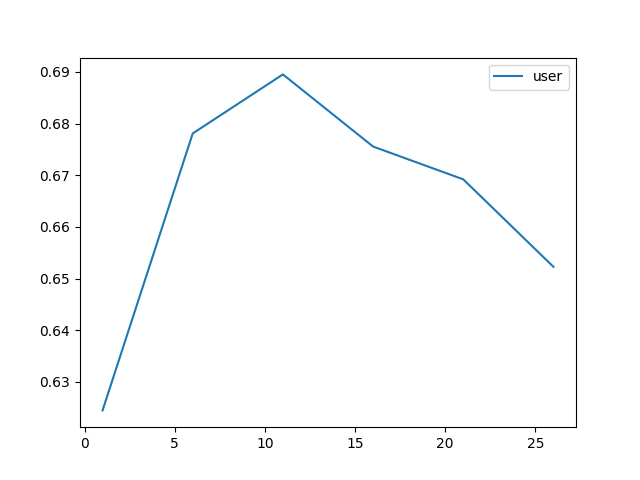
\includegraphics[width=\linewidth]{../starter_code/figs/knn_user.png}
                \end{minipage}\hfill
                \begin{minipage}{0.5\linewidth}
                    \center
                    \begin{tabular}{c|c}
                        $k$ & Validation Accuracy \\\hline
                        1 & 0.6244707874682472\\
                        6 & 0.6780976573525261\\
                        11 & 0.6895286480383855\\
                        16 & 0.6755574372001129\\
                        21 & 0.6692068868190799\\
                        26 & 0.6522720858029918
                    \end{tabular}
                \end{minipage}
            \item The best value of $k$ for user-based collaborative filtering is $k^*=11$.
            \item For distance by item, we have:

                \noindent
                \begin{minipage}{0.5\linewidth}
                    \centering
                    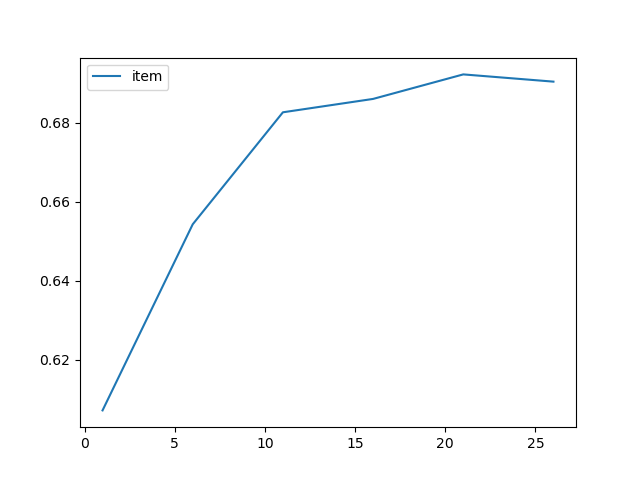
\includegraphics[width=\linewidth]{../starter_code/figs/knn_item.png}
                \end{minipage}\hfill
                \begin{minipage}{0.5\linewidth}
                    \center
                    \begin{tabular}{c|c}
                        $k$ & Validation Accuracy \\\hline
                        1 & 0.607112616426757\\
                        6 & 0.6542478125882021\\
                        11 & 0.6826136042901496\\
                        16 & 0.6860005644933672\\
                        21 & 0.6922099915325995\\
                        26 & 0.69037538808919
                    \end{tabular}
                \end{minipage}
                And the best value of $k$ for item-based collaborative filtering is $k^*=21$.

                An assumption made here is that questions that were answered similarly are equal in difficulty. This might not always be case, keeping in mind that questions may span completely different subjects and there are only so many ways to pose a question. A question in a introductory chemistry quiz may be answered similarly to a graduate-level statistics question if both of them are multiple-choice.
            \item For the chosen values of $k$: $k^*_{\text{user}}=11$, $k^*_{\text{item}}=21$, we find that the test accuracy is 0.68416596105 and 0.68165274090, respectively. So the user-based collaborative filtering performs better.
            \item Here are two limitations of KNN for this task:
                \begin{itemize}
                    \item KNN is slow. Even with only 542 items and 1774 users it takes a while to predict.
                    \item Using Euclidean distance, we consider distances in all dimension to be equal. For example if A and B's math skills are very different but english, physics, and other subjects are similar, the KNN will still predict A's math question similar to B's math questions (since skill in math is treated equally with other subjects).
                \end{itemize}

        \end{enumerate}
        
    \item In this approach, we use Item Response Theory to predict students' correctness to diagnostic questions.
        \begin{enumerate}[label=(\alph*)]
            \item Here, we derive an expression for the log-likelihood corresponding to this model and its derivative with respect to the user-ability and question-difficulty parameters. 
                \begin{align*}
                    \mc L(\mbf C|\bs\theta,\bs\beta) &= \sum_{i=1}^{N}{\sum_{j=1}^{J}{P(c_{ij}=1|\theta_i,\beta_j)^{c_{ij}}(1-P(c_{ij}=0|\theta_i,\beta_j))^{1-c_{ij}}}} \\
                    \ell(\mbf C|\bs\theta, \bs\beta) &= \sum_{i=1}^{N}{\sum_{j=1}^{J}{c_{ij}\log(P(c_{ij}=1|\theta_i,\beta_j))+(1-c_{ij})\log(1-P(c_{ij}=0|\theta_i,\beta_j))}} \\
                                                     &= \sum_{i=1}^{N}{\sum_{j=1}^{J}{\left(c_{ij}\left[(\theta_i-\beta_j)-\log(1+\exp(\theta_i-\beta_j))\right]+(1-c_{ij})\log \left(\frac{1}{1+\exp(\theta_i-\beta_j)}\right)\right)}} \\
                                                     &= \sum_{i=1}^{N}{\sum_{j=1}^{J}{\left(c_{ij}(\theta_i-\beta_j)-\log(1+\exp(\theta_i-\beta_j))\right)}} \\
                                                     &= \sum_{i\colon (i, j)\in C}{\sum_{j\colon (i, j)\in C}{\left(c_{ij}(\theta_i-\beta_j)-\log(1+\exp(\theta_i-\beta_j))\right)}} \\
                    \pdv{\ell}{\theta_i} &= \sum_{j\colon (i, j)\in C}{c_{ij}}-\sum_{j\colon (i, j)\in C}{\frac{\exp(\theta_i-\beta_j)}{1+\exp(\theta_i-\beta j)}} \\
                    \pdv{\ell}{\beta_j} &= \sum_{i\colon (i, j)\in C}{-c_{ij}} + \sum_{i\colon (i, j)\in C}{\frac{\exp(\theta_i-\beta_j)}{1+\exp(\theta_i-\beta j)}}
                \end{align*}
            \item We found the following hyperparameters to be the best:
                \begin{itemize}
                    \item learning rate=0.016
                    \item number of iterations=10 
                \end{itemize}
                Here is the plot of log-likelihoods on the training and validation data:
                \begin{center}
                    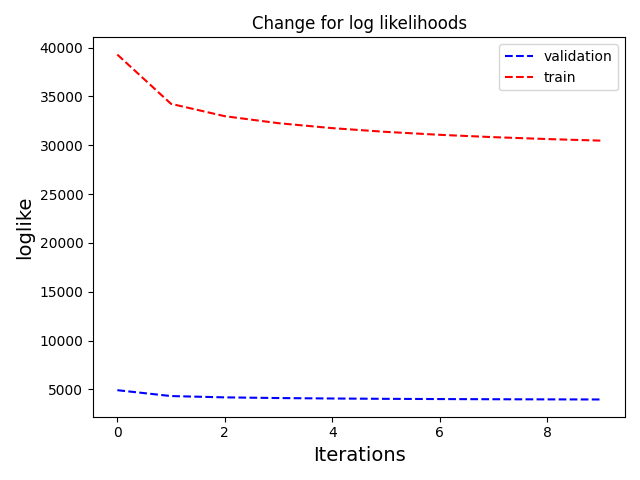
\includegraphics[width=0.6\linewidth]{../starter_code/irt_output/myplot.png}
                \end{center}
            \item For the same hyperparameters, we achieved:
                \begin{itemize}
                    \item Final validation accuracy: 0.7064634490544736
                    \item Final test accuracy: 0.7039232289020604
                \end{itemize}
            \item The plot is shown below. It shows the probability of correct response $P(c_{ij}|\theta_i,\beta_j)$ as a function of $\theta_i$, which represents the $i$-th student's ability. For each fixed question, the relationship between $P(c_{ij}|\theta_i,\beta_j)$ and $\theta$ follows the sigmoid function \[
                    P(c_{ij}|\theta_i,\beta_j)=\frac{\exp(\theta_i-\beta_j)}{1+\exp(\theta_i-\beta_j)}
            \] 
            There is a positive relationship between $P(c_{ij}|\theta_i,\beta_j)$ and $\theta$. It makes sense that a student having greater ability would be more likely to answer a question correctly if we hold the question difficulties constant.

            Also, notice that different questions have different correctness probabilities if we hold the students' abilities constant. For instance, the curve for the question with ID 3 is above the curve for the question with ID 4, indicating that the former is more likely to be correctly answered by students with equal ability compared to the latter question, which is comparatively harder.
                \begin{center}
                    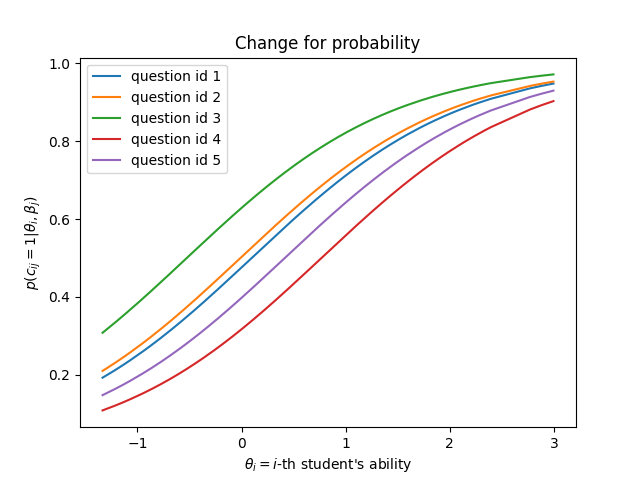
\includegraphics[width=0.6\linewidth]{../starter_code/figs/irt.png}
                \end{center}
        \end{enumerate}
        
    \item In this approach, we use neural networks. %both matrix factorization and neural networks.
        \begin{enumerate}[label=(\roman*)]
            \addtocounter{enumii}{1}
            %\item 
                %Matrix Factorization \textcolor{red}{remove this if we are not using it}
                %\begin{enumerate}[label=(\alph*)]
                %    \item d
                %\end{enumerate}
            \item Neural Networks
                \begin{enumerate}[label=(\alph*)]
                    \item Here are some differences between the neural network autoencoder and ALS:
                        \begin{enumerate}
                            \item The parameterizations of the problems are different. In the neural network, we're training the weights of the activation functions $g, h$ to minimize the squared error loss which is computed by passing the input through the two-layer autoencoder. In ALS, we're training the vectors $\mbf u,\mbf z$, reconstructing the matrix, and then computing the squared error loss by the reconstruction error.
                            \item We can use backpropagation in neural networks, but we can't do the same for the ALS optimization problem.
                            \item We use different activation functions. In ALS, we classify predictions as correct if they're above 0.5 and incorrect otherwise, but we allow the predictions to go above 1 (consider the case where a question was very hard for many people, then the term would become very large). In the neural network, we use a sigmoid activation function for each of the layers, ensuring that the output numbers are valid probabilities between 0 and 1.
                            %\item In ALS, we are only iterating over the observed values. In neural networks, we don't care about what's observed and what's not; we use only the fact that the best possible $K$-dimension linear subspace is the PCA substance, achieved by setting $\mbf W_1=\mbf U^\top,\mbf W_2=\mbf U$ \cite{pcaapplications}.
                        \end{enumerate}
                    \item See \texttt{neural\_network.py}
                    \item We trained models using a variety of hyperparameters and found that a good combination was $k$ (latent dim.) = 10, learning rate = 0.01, epochs = 100. This achieved a training cost of 8376.565430	 and validation accuracy of 0.6891052780129834.
                    %\begin{center}
                    %    \begin{tabular}{c|c|c|c|c|c}
                    %        $k$ (latent dim.) & learning rate & epochs & $\lambda$ (penalty) & train cost & val. accuracy \\\hline
                    %        10 & 0.01 & 100 & 0.1 & 10545.283 & 0.68784 \\
                    %        10 & 0.01 & 100 & 0.5 & 19321.324219 & 0.69038 \\
                    %        50 & 0.05 & 10  & 0.5 & 17700.197 & 0.690799 \\
                    %        100 & 0.01 & 50 & 0.1 & 7667.879 & 0.68246 \\
                    %        100 & 0.05 & 10 & 0 & 6923.447 & 0.68346 \\
                    %        200 & 0.01 & 50 & 0.1 & 6638.1338 & 0.6782388 \\
                    %        200 & 0.01 & 50 & 0.5 & 16577.74 & 0.6745696 
                    %    \end{tabular}
                    %\end{center}
                    %Setting $k=500$ led to comparatively low validation accuracy (mean average of $0.651150$). For the other values of $k$, there weren't discernible correlations between the choice of hyperparameters and the performance of the model; the lower training cost and higher validation accuracy can probably be attributed to luck. We choose $k^*=10$ since the combination on the second row has a validation accuracy of 0.69038.
                    \item The final test accuracy was 0.6838837143663562.

                    \begin{center}
                        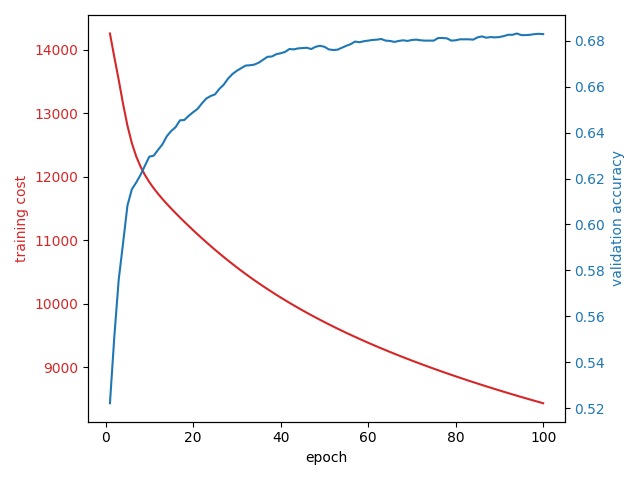
\includegraphics[width=0.6\linewidth]{../starter_code/nn_output/3d.png}
                    \end{center}
                \item We chose $\lambda=0.1$ and all of the other hyperparameters remain the same. This results in a final validation accuracy of 0.6830369743155518
and a test accuracy of 0.6850127011007621.

                    \begin{center}
                        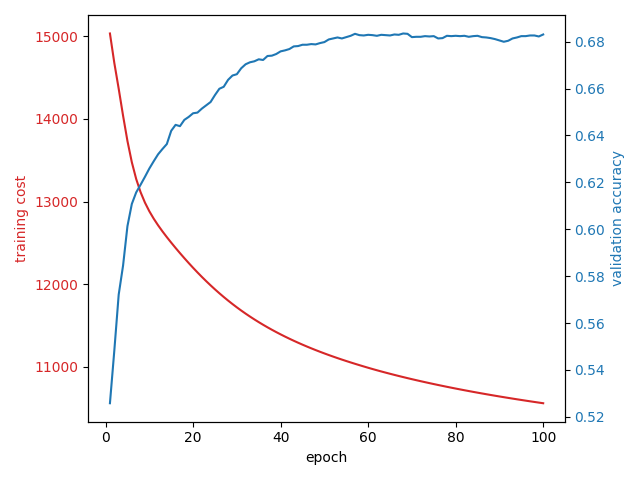
\includegraphics[width=0.6\linewidth]{../starter_code/nn_output/3e.png}
                    \end{center}
                \end{enumerate}
        \end{enumerate}
    \item For our ensemble, we decided to use the following base models:
        \begin{enumerate}
            \item Item response theory model with hyperparameters: 10 iterations, 0.016 learning rate
            \item ALS matrix factorization with hyperparameters: latent dimension 35, 0.01 learning rate, 500000 iterations
            \item Random-splitting decision tree with $\log_2n$ levels, i.e. it splits a node to be an internal node if there is at least 2 samples at that node.
        \end{enumerate}
        We also bootstrapped the training set by sampling three times with replacement, and then using one of those datasets for each of the models. The decisions of the three models are weighted equally, so the bagged model prediction was given by \[
            \frac{\sum_{d\in \text{data}}{\left(\text{pred}_{\text{IRT}}(d)+\text{pred}_{\text{ALS}}(d)+\text{pred}_{\text{tree}}(d)\right)}}{3}
        \] and then compared to the usual 0.5 threshold.

        The objective and reason why we employed this ensembling process was because we found it quite hard to push past the $\sim 0.68-0.70$ test accuracy threshold using only one base model without drastically overfitting on the training data. It was apparent through tuning of hyperparameters, especially for the neural network, that improvements may have been due to chance and that the models wouldn't generalize well to new data. In adding more predictors via bagging, we reduce the variance and reduce overfitting, but increase the bias. 

        The results of our implementation are as follows:
        \begin{itemize}
            \item Validation accuracy: 0.7039232289020604
            \item Test accuracy: 0.694609088343212
        \end{itemize}
\end{enumerate}

\newpage
\section{Part B}
\begin{enumerate}[label=\arabic*.]
    \item We chose to improve upon our matrix factorization model because our testing in Part A yielded the most promising results with this model on the test data. 

        We amended the initial squared error loss; the new objective function we aimed to minimize is \cite{netflix}: \[
            \mathcal{J}_{b\lambda} := \frac{1}{2}\sum_{(n, m)\in O}{\left(C_{nm}-\left(\mbf u_n^\top \mbf z_m+\mbf b_{u_n}+\mbf b_{z_m}+\mu\right)\right)^2+\lambda \left(\mbf u_n^\top\mbf u_n+\mbf z_m^\top\mbf z_m+\mbf b_{u_n}+\mbf b_{z_m}\right)}
        \] where:
        \begin{itemize}
            \item $\mbf b_{u_n}$ is a bias term for user $n$. It is initialized to the ratio of number of answers by user $n$ to the total amount of observed data, i.e. \[
                    \mbf b_{u_n} := \frac{\left|\left\{(n, m)\in O\right\}\right|}{\text{total observed data}}
            \] 
            \item $\mbf b_{z_m}$ is a bias term for question $m$. It is initialized to the ratio of number of answers for question $m$ to the total amount of observed data, i.e. \[
                    \mbf b_{z_m} := \frac{\left|\left\{(n, m)\in O\right\}\right|}{\text{total observed data}}
            \] 
            \item $\mu$ is a scalar initialized to the ratio of correct data to the total amount of observed data, i.e. \[
            \mu := \frac{\text{correct answers}}{\text{total observed data}}
            \] 
            \item $\lambda$ is a penalty/regularization hyperparameter
        \end{itemize}

        We added weight regularization to the gradient descent method of optimizing the loss in our alternating least squares matrix factorization algorithm and bias/weight terms to every user and question. Intuitively, it is useful to weigh the users and questions that have more responses higher because they give more information, which is very useful when dealing with our issue of sparsity in the data. To start, given $k$, $\mbf u$ and $\mbf z$ were initialized by taking a uniform random sample of shape $(\text{\# user/question}, k)$ over $\left[0, \left\lfloor \frac{1}{\sqrt k}\right\rfloor\right]$. Then, we obtained the following update rules for $\operatornamewithlimits{argmin}_{\mbf u,\mbf z} \mathcal{J}_{b\lambda}$ via stochastic gradient descent:
        \begin{align*}
            \mbf u_n' &\gets \mbf u_n-\alpha \left(-\left(c_{nm}-\mu-\mbf b_{u_n}-\mbf b_{z_m}-\mbf u^\top\mbf z\right)\mbf z+\lambda\mbf u_n\right) \\
            \mbf z_m' &\gets \mbf z_m-\alpha \left(-\left(c_{nm}-\mu-\mbf b_{u_n}-\mbf b_{z_m}-\mbf u^\top\mbf z\right)\mbf u+\lambda\mbf z_m\right) \\
            \mbf b_{u_n}' &\gets \mbf b_{u_n}-\alpha \left(-(c_{nm}-\mu-\mbf b_{u_n}-\mbf b_{z_m}-\mbf u^\top\mbf z)+\lambda\mbf b_{u_n}\right) \\
            \mbf b_{z_m}' &\gets \mbf b_{z_m}-\alpha \left(-(c_{nm}-\mu-\mbf b_{u_n}-\mbf b_{z_m}-\mbf u^\top\mbf z)+\lambda\mbf b_{z_m}\right)
        \end{align*}
        For all of the new models, we opted to early-stop at 3000000 (3 million) iterations in order to prevent overfitting to the training data, since in the plots in the third question of this section, we saw that the validation loss began to increase past this point. Furthermore, we took this training approach for six models, each trained differently with corresponding $k$ values of $[40, 50, 60, 70, 80, 90]$. We did this in an attempt to reduce overfitting to the training data, reducing variance, and also increasing the bias. Their predictions were averaged and then compared to the usual threshold of 0.5, classifying the $(\text{user}, \text{question})$ pair as correct if it was greater. Another objective of this approach was to hopefully increase test performance by weighing more important points higher.
    \item In this section, we illustrate several ideas about our model. 

        \begin{minipage}[c]{0.35\linewidth}
            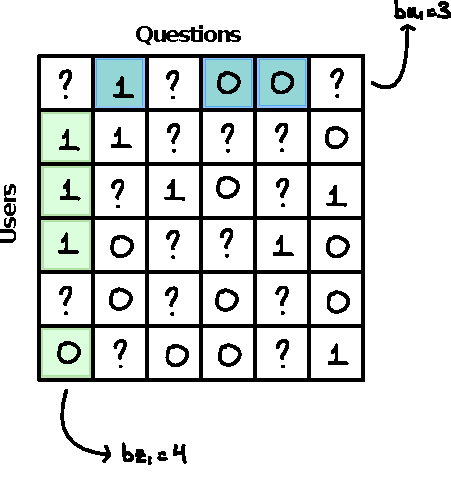
\includegraphics[width=\linewidth]{./images/train_sparse_bias.pdf}
            \captionof{figure}{Sparse train matrix showing how the user and question biases are initialized}
            \label{sparsebias}
        \end{minipage}\hfill
        \begin{minipage}[c]{0.6\linewidth}
            \begin{minipage}{0.4\linewidth}
                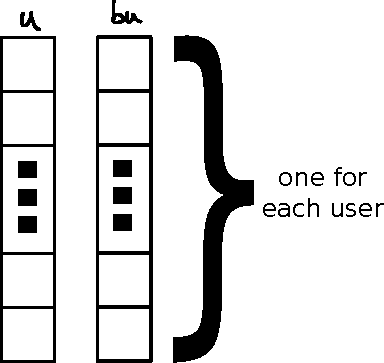
\includegraphics[width=\linewidth]{./images/bias_user.pdf}
            \end{minipage}\hfill
            \begin{minipage}{0.4\linewidth}
                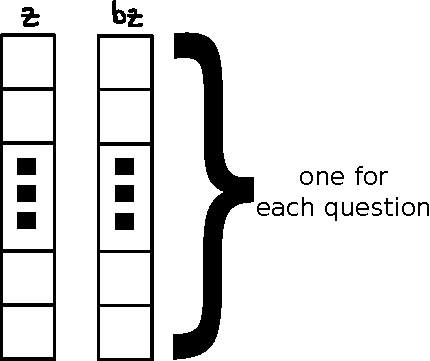
\includegraphics[width=\linewidth]{./images/bias_question.pdf}
            \end{minipage}
            \captionof{figure}{Parameters $\mbf u,\mbf z$ we aim to optimize for, and biases $\mbf b_u, \mbf b_z$}
            \label{biases}
        \end{minipage}

        Firstly, the model's goal is to take the training matrix in Figure~\ref{sparsebias} and complete it so that the unobserved entries, marked `?', are predicted. The $N\times J$ matrix can split into two matrices $\mbf u$ (size $N\times k$) and $\mbf z$ (size $J\times k$), where $k$ is the latent dimension hyperparameters, as shown in Figure~\ref{biases} for $k=1$. The reconstruction works by multiplying $\mbf u,\mbf z$:
        \[
            \underbrace{\mbf u}_{N\times k}\underbrace{\mbf z^\top}_{k\times J}=\underbrace{\text{reconstructed matrix}}_{N\times J}
        \] 
        For bootstrapping the training data, we sampled the indices of the training data with replacement so that duplicates would be included, meaning some points could be represented more than once. This is shown in Figure~\ref{bagging}.

        \begin{center}
            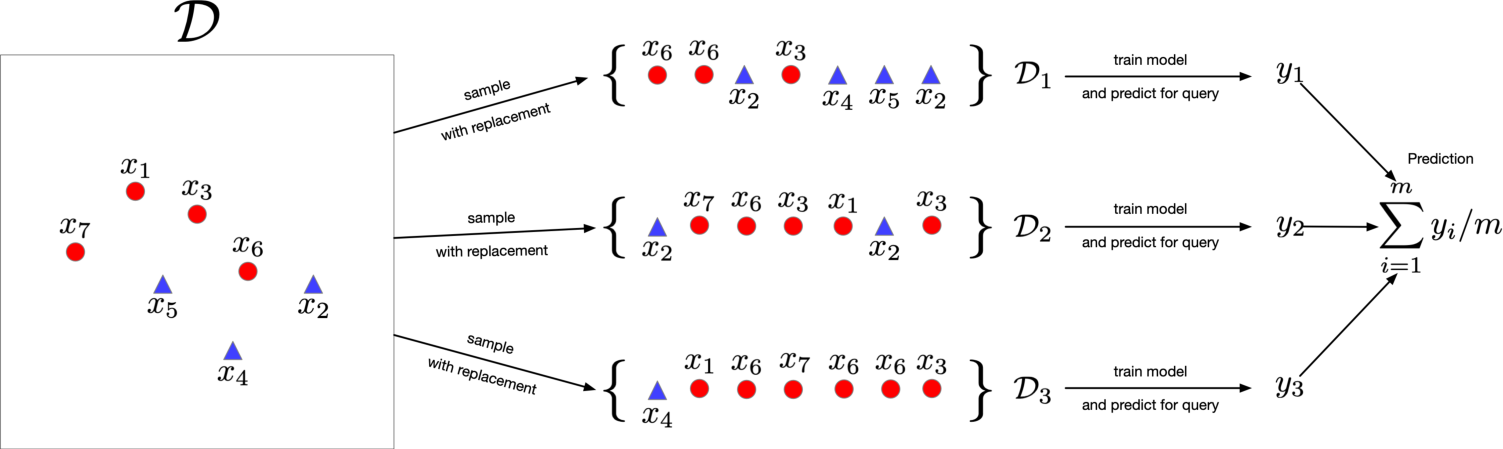
\includegraphics[width=\linewidth]{./images/bagging.pdf}
            \captionof{figure}{Illustration of bagging approach for the various matrix factorization models, taking the average of the predictions for the base models as the overall prediction~\cite{bagginglec}.}
            \label{bagging}
        \end{center}

    \item In this section, we compare the performance of our model using the same initialization of $\mbf u,\mbf z$, learning rate, and number of iterations with the baseline ALS matrix completion model. We will consider the training loss and prediction accuracy on the test data to see if our changes were useful. 

        Below, the left plots in Figures \ref{nobiasreg40}, \ref{nobiasreg50}, \ref{nobiasreg60}, \ref{nobiasreg70}, \ref{nobiasreg80}, \ref{nobiasreg90} show the validation loss as the original models without bias and regularization are trained for 1 million iterations. The right plots in Figures \ref{withbiasreg40}, \ref{withbiasreg50}, \ref{withbiasreg60}, \ref{withbiasreg70}, \ref{withbiasreg80}, \ref{withbiasreg90} show the validation loss as the new models with bias and regularization are trained for 4 million iterations. Note that the validation losses are on different scales due to the addition of various terms in the new model, but the general trend is the same. The models with bias and regularization have a very erratic trend. 

        The corresponding validation and test accuracies of the original models are as follows:

        \begin{center}
            \begin{tabular}{c|c|c}
                $k$ & validation accuracy & test accuracy \\\hline
                40 & 0.7085802991814846 & 0.7087214225232854 \\
                50 & 0.7056167090036692 & 0.7061812023708721 \\
                60 & 0.707310189105278 & 0.707310189105278 \\
                70 & 0.7050522156364663 & 0.7084391758396839 \\
                80 & 0.707310189105278 & 0.7061812023708721 \\
                90 & 0.7061812023708721 & 0.703076488851256 \\
            \end{tabular}
        \end{center}
        The validation and test accuracies of our final, bootstrapped with bias and weight regularization were 0.7068868190798758 and 0.7058989556872707, respectively.

        Thus, the performance did not improve by much but the model is more generalizable because we bagged the models. This more or less falls in line with our expectations; we don't expect bagging to increase the accuracy. 
        

        %723.0853628041474 200000 0.2
        %701.8524423993288 300000 0.3
        %689.867261692518 400000 0.4
        %687.9347706896374 500000 0.5
        %686.0736001353497 600000 0.6
        %685.803993746787 700000 0.7
        %683.3203583586919 800000 0.8
        %682.7726872114937 900000 0.9
        %4591.29994549652
        %validation 0.7054755856618685
        %test 0.7090036692068868
        %722.931326530254 200000 0.2
        %698.4321940059158 300000 0.3
        %688.9629155491974 400000 0.4
        %685.9274410406473 500000 0.5
        %683.001712361564 600000 0.6
        %682.7849629871617 700000 0.7
        %682.1546202100534 800000 0.8
        %681.9753838713801 900000 0.9
        %4524.5573054474435
        %validation 0.7085802991814846
        %test 0.7087214225232854
        %723.9602064846085 200000 0.2
        %700.2439442446165 300000 0.3
        %688.7425829765167 400000 0.4
        %685.8680326367414 500000 0.5
        %682.8818874671783 600000 0.6
        %682.0543526570382 700000 0.7
        %683.2722794983586 800000 0.8
        %682.8368087209143 900000 0.9
        %4501.322347696243
        %validation 0.7056167090036692
        %test 0.7061812023708721
        %724.6613737701703 200000 0.2
        %701.4008805446995 300000 0.3
        %690.1703123750199 400000 0.4
        %686.0837684751644 500000 0.5
        %684.1097370354307 600000 0.6
        %683.0951345165043 700000 0.7
        %681.0175114328564 800000 0.8
        %681.9032852657122 900000 0.9
        %4500.400724891759
        %validation 0.707310189105278
        %test 0.707310189105278
        %721.516649055351 200000 0.2
        %699.5281297311434 300000 0.3
        %689.4315273326175 400000 0.4
        %685.7180784349583 500000 0.5
        %682.3861392440592 600000 0.6
        %682.0942839941125 700000 0.7
        %681.5440144303245 800000 0.8
        %682.1406789905474 900000 0.9
        %4488.436588200986
        %validation 0.7050522156364663
        %test 0.7084391758396839
        %723.3763617468431 200000 0.2
        %699.6201952322318 300000 0.3
        %689.8165425132408 400000 0.4
        %686.1825155552731 500000 0.5
        %683.1949544455069 600000 0.6
        %681.5914503098212 700000 0.7
        %679.9392617976873 800000 0.8
        %681.6994286032927 900000 0.9
        %4475.792925393139
        %validation 0.707310189105278
        %test 0.7061812023708721
        %723.8622142246405 200000 0.2
        %698.0150273562035 300000 0.3
        %687.6178765346813 400000 0.4
        %684.8084341198843 500000 0.5
        %684.2818883501437 600000 0.6
        %682.6377618264978 700000 0.7
        %681.5118969031089 800000 0.8
        %681.6140776557189 900000 0.9
        %4459.632367593904
        %validation 0.7061812023708721
        %test 0.703076488851256


        \begin{minipage}{0.49\linewidth}
            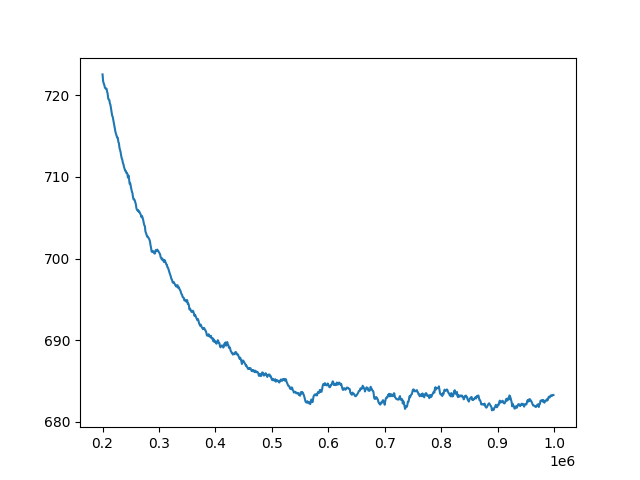
\includegraphics[width=\linewidth]{../starter_code/figs/sgd_wo_k_40.png}
            \captionof{figure}{No bias \& regularization, $k=40$}
            \label{nobiasreg40}
        \end{minipage}\hfill
        \begin{minipage}{0.49\linewidth}
            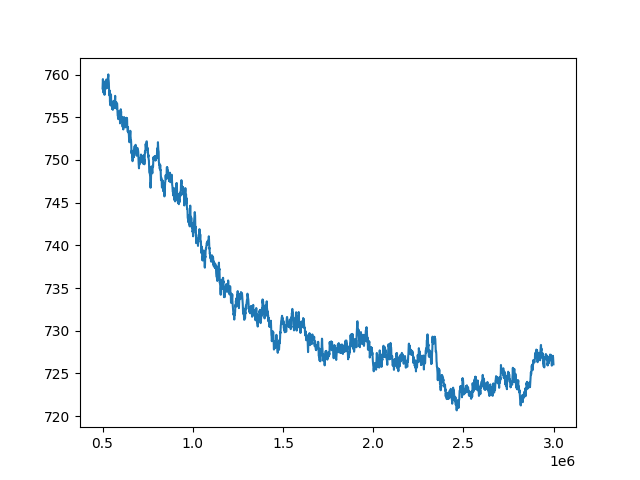
\includegraphics[width=\linewidth]{../starter_code/figs/sgd_k40.png}
            \captionof{figure}{With bias \& regularization, $k=40$}
            \label{withbiasreg40}
        \end{minipage}\hfill
        \begin{minipage}{0.49\linewidth}
            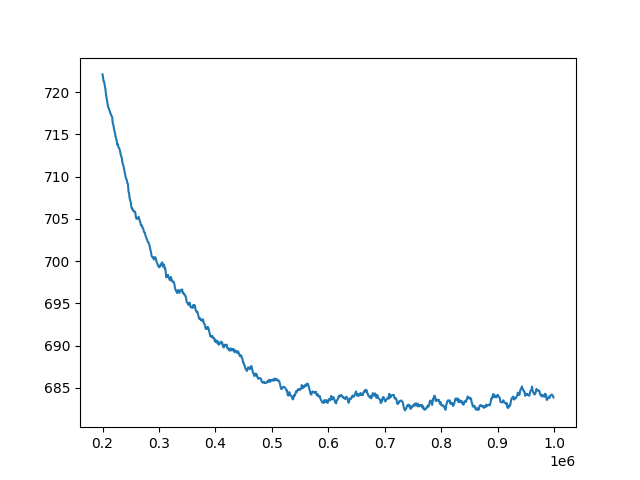
\includegraphics[width=\linewidth]{../starter_code/figs/sgd_wo_k_50.png}
            \captionof{figure}{No bias \& regularization, $k=50$}
            \label{nobiasreg50}
        \end{minipage}\hfill
        \begin{minipage}{0.49\linewidth}
            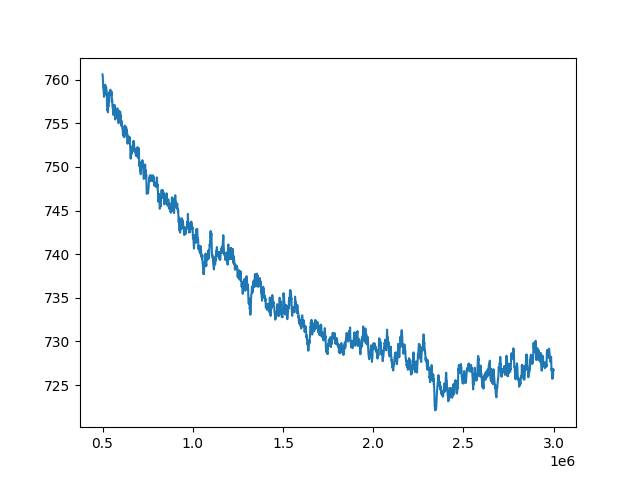
\includegraphics[width=\linewidth]{../starter_code/figs/sgd_k50.png}
            \captionof{figure}{With bias \& regularization, $k=50$}
            \label{withbiasreg50}
        \end{minipage}\hfill
        \begin{minipage}{0.49\linewidth}
            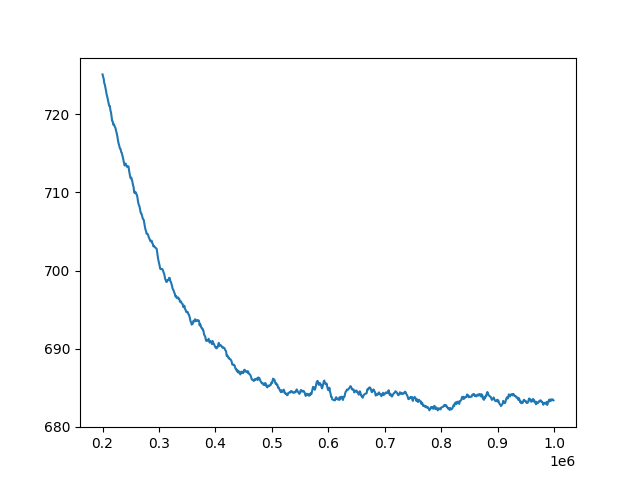
\includegraphics[width=\linewidth]{../starter_code/figs/sgd_wo_k_60.png}
            \captionof{figure}{No bias \& regularization, $k=60$}
            \label{nobiasreg60}
        \end{minipage}\hfill
        \begin{minipage}{0.49\linewidth}
            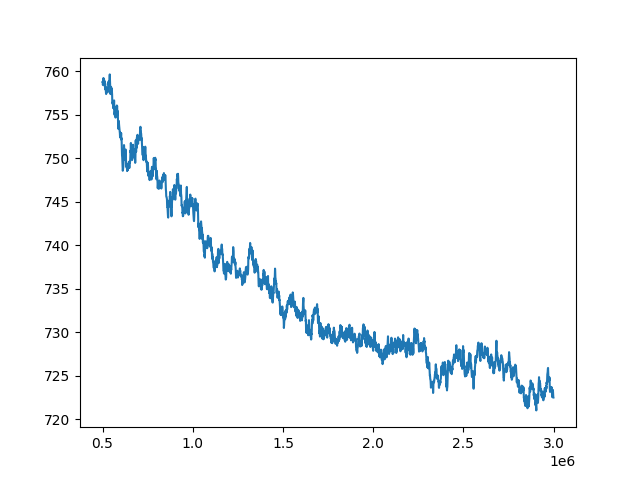
\includegraphics[width=\linewidth]{../starter_code/figs/sgd_k60.png}
            \captionof{figure}{With bias \& regularization, $k=60$}
            \label{withbiasreg60}
        \end{minipage}\hfill
        \begin{minipage}{0.49\linewidth}
            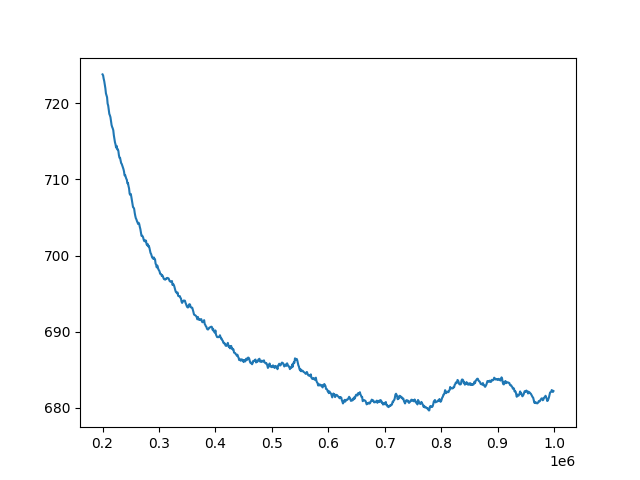
\includegraphics[width=\linewidth]{../starter_code/figs/sgd_wo_k_70.png}
            \captionof{figure}{No bias \& regularization, $k=70$}
            \label{nobiasreg70}
        \end{minipage}\hfill
        \begin{minipage}{0.49\linewidth}
            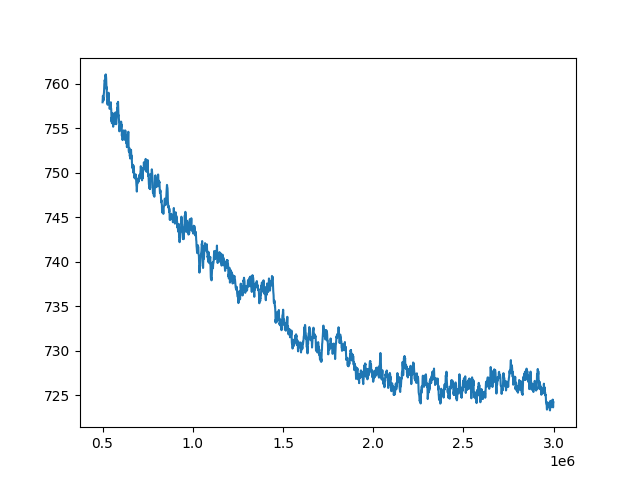
\includegraphics[width=\linewidth]{../starter_code/figs/sgd_k70.png}
            \captionof{figure}{With bias \& regularization, $k=70$}
            \label{withbiasreg70}
        \end{minipage}\hfill
        \begin{minipage}{0.49\linewidth}
            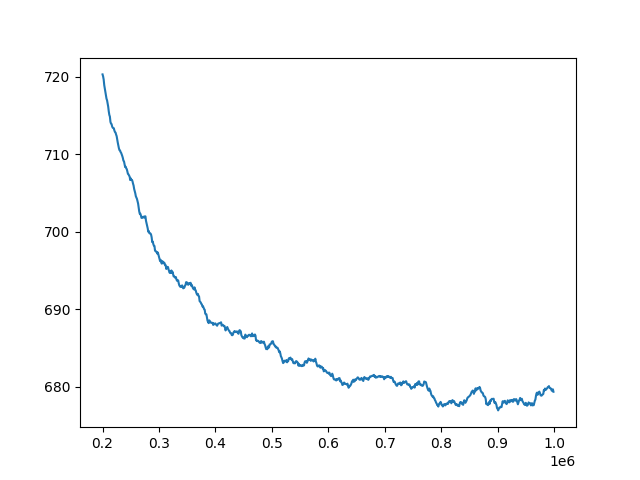
\includegraphics[width=\linewidth]{../starter_code/figs/sgd_wo_k_80.png}
            \captionof{figure}{No bias \& regularization, $k=80$}
            \label{nobiasreg80}
        \end{minipage}\hfill
        \begin{minipage}{0.49\linewidth}
            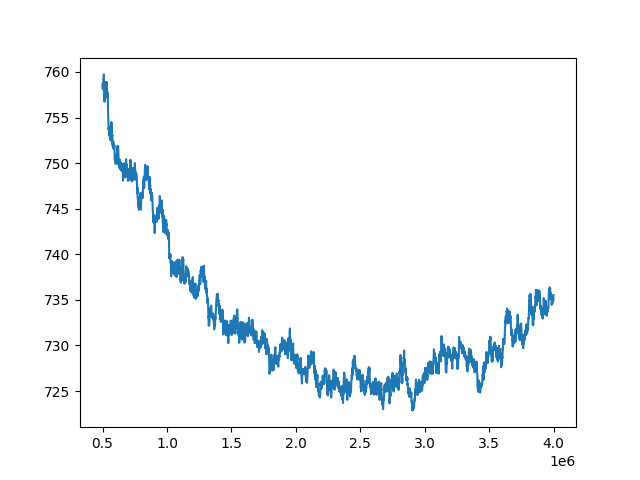
\includegraphics[width=\linewidth]{../starter_code/figs/sgd_k80.png}
            \captionof{figure}{With bias \& regularization, $k=80$}
            \label{withbiasreg80}
        \end{minipage}\hfill
        \begin{minipage}{0.49\linewidth}
            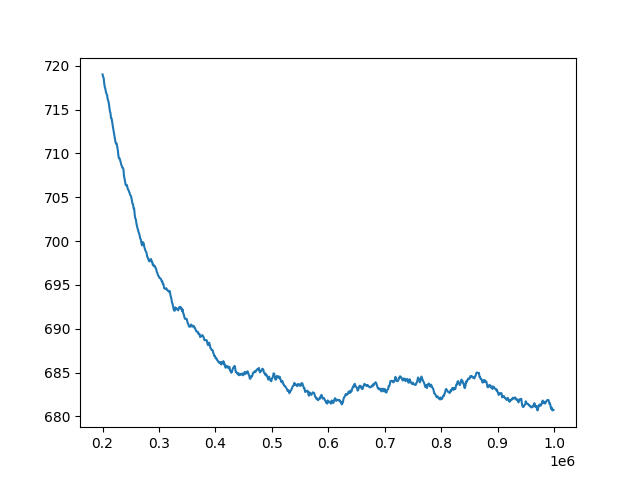
\includegraphics[width=\linewidth]{../starter_code/figs/sgd_wo_k_90.png}
            \captionof{figure}{No bias \& regularization, $k=90$}
            \label{nobiasreg90}
        \end{minipage}\hfill
        \begin{minipage}{0.49\linewidth}
            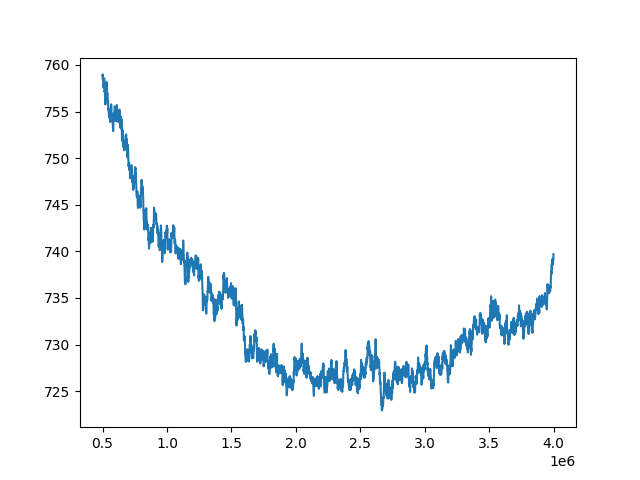
\includegraphics[width=\linewidth]{../starter_code/figs/sgd_k90.png}
            \captionof{figure}{With bias \& regularization, $k=90$}
            \label{withbiasreg90}
        \end{minipage}
    \item Our method may not perform optimally if the weights are roughly equal, since there wouldn't be a gain in this instance. It wouldn't perform badly -- it would just take awhile to train. The addition of weight regularization means that it makes many more iterations to train the models, and if the overall performance remains the same, then there is no point in incorporating the biases and weight regularization. Another shortcoming is the lack of appropriate metadata that could help with weighing the features. 

        A major limitation of matrix factorization is over-specialization. The new prediction for a particular student is based on the student's past performance; when a new question appears, a student who's historically achieved high grades is predicted to be more likely to answer it correctly. This may not always be the case, because students with poor grades in the past may improve their study habits to perform well in the future. In addition, the data we used doesn't sufficient data to represent the student's ability in terms of other academic competencies.

        In other words, we don't have enough data, and that's likely the reason why most models we have attain only around 70\% accuracy on the training, validation, and test sets. 

        One way to improve the first limitation is that we could try to add some randomness to the model, changing the original squared error loss to be \[
            \mathcal{J}_{b\lambda\varepsilon} := \frac{1}{2}\sum_{(n, m)\in O}{\left(C_{nm}-\left(\mbf u_n^\top \mbf z_m+\mbf b_{u_n}+\mbf b_{z_m}+\mu+\varepsilon\right)\right)^2+\lambda \left(\mbf u_n^\top\mbf u_n+\mbf z_m^\top\mbf z_m+\mbf b_{u_n}+\mbf b_{z_m}\right)}
        \] 
        where $\varepsilon\sim \mathcal N(0,\sigma^2)$ is a hyperparameter we select using the validation set in order to promote/simulate `improvements' in students' performance. With this definition, most students would have small improvements ($\varepsilon_i$ would be near the mean of 0), but some may increase/decrease in ability drastically ($\varepsilon_i$ would be at the tails of the normal distribution).

        The second limitation could be addressed by using the question metadata, which contains information about the question subject. It might be useful to introduce an additional constant $s_{ij}$ which represents the student's ability for a certain subject. For example, let's assume student $i$ answers question $j$, where question $j$ is a geometry question. Then we could define this term to be a function of the number of geometry questions the student has answered correctly: \[
            s_{ij}=f(\text{\# of geometry questions the student has answered correctly})
        \]
        It would be interesting to see if there are other datasets available for this problem and to see if there are any class-wide breakthroughs in models for this problem, just like there was for the Netflix recommendation system problem. 
\end{enumerate}

\nocite{*}
\printbibliography[title={\section{References}}]
\end{document}
